\begin{center}
    \addcontentsline{toc}{section}{ПРАКТЫЧНАЯ РЭАЛІЗАЦЫЯ}
    \section*{ГЛАВА 2. \\ ПРАКТЫЧНАЯ РЭАЛІЗАЦЫЯ}
\end{center}

\renewcommand{\floatpagefraction}{.8}%

У гэтым раздзеле я хачу апісаць дзве практычныя часткі, зробленыя мной.
Першая - серыя эксперыментаў над выманнем асаблівых кропак, падлікам іх дэскрыптараў і
пошукам адпаведнасцяў паміж дзвюма выявамі з аднаго набору.
Другая - апісанне распрацаванага праграмнага забеспячэння, якое выконвае ўвесь цыкл рэканструкцыі,
пабудаванае на аснове бібліятэкі \cite{theia-sfm}.

\vspace{5mm}

\addcontentsline{toc}{subsection}{Эксперыменты над асаблівасцямі выяваў}
\subsection*{2.1 Эксперыменты над спосабамі вымання асаблівых кропак, іх апісання і пошуку}

Практычна-даследніцкая частка маёй працы - параўнанне розных дэтэктараў, дэскрыптараў, тыпаў ключавых кропак
на рознага кшталту дадзеных, пошук узаемасувязі паміж тыпам пачатковых дадзеных і якасцю вынікаў, у залежнасці
ад прымененых алгарытмаў.

\vspace{5mm}

Для правядзення эксперыментаў я выбраў 4 набора дадзеных па 2 выявы. Крытэрам выбара была разнастайнасць: выявы павінны быць моцна альбо
слаба тэкстураванымі; адрознівацца паваротам, паралельным пераносам альбо выбарам іншага вугла камеры і г.д., яскравайвыраджанай
альбо аднастайнай каляровай гамай. Далей ідзе кароткае апісанне кожнага з набораў.

\begin{itemize}
    \item \textit{church:} два фотаздымкі царквы ў Швейцарыі, зробленыя з БПЛА.
    Маюць яскравую выраджанасць асобных аб'ектаў, у першую чаргу будынкаў. Гл. малюнкі \ref{fig:church}.
    \item \textit{fountain:} два фотаздымкі фантана, зробленыя пад розным вуглом.
    Пераважвае адзіная каляровая гамма, выявы слаба тэкстураваныя. Гл. малюнак \ref{fig:fountain}.
    \item \textit{ellis:} два фотаздымкі з выглядам на Манхэтэн, прыблізна палову
    кожнага здымка займае аднастайныя тэкстуры: вада, дарога. Аб'екты, якія знаходзяцца
    на абодвух выявах, моцна адрозніваюцца масштабам. Гл. малюнак \ref{fig:ellis}.
    \item \textit{grass:} два фотаздымкі беларускай сельскай мясцовасці зробленыя з БПЛА.
    Большая частка абодвух выяваў занятыя аднастайнай, практычна алнакаляровай тэкстурай. Гл. малюнак \ref{fig:grass}
\end{itemize}

Усе выявы былі папярэдне прыведзеныя да параўнальных памераў: вышыня кожнай выявы склала 640 пікселяў,
шырыня вылічвалася з захаваннем прапорцыяў.

Усе эксперыменты праводзіліся пры аднолькавых умовах, на камп'ютары з усталяванай ubuntu 16.04 з 2gb RAM на аднаядравым працэсары.
Рэалізацыі алгарытмаў браліся з бібліятэкі камп'ютарнага зроку з адкрытым зыходным кодам OpenCV.

Для кожнага набора дадзеных падлікі прадстаўленыя ў дзвюх табліцах.
У першай табліцы ідзе апісанне часавых характарыстыкаў дэтэкцыі кропак і падліку іх апісання рознымі алгарытмамі.
У другой - часавыя і колькасныя характарыстыкі алгарытмаў пошуку адпаведнасцяў паміж дзвюма выявамі з набора.

Вынікі эксперыментаў для дадзеных \textit{church} прыведзеныя ў табліцах \ref{table:church-kp} i \ref{table:church-matching},
\textit{fountain} - \ref{table:fountain-kp} i \ref{table:fountain-matching},
\textit{ellis} - \ref{table:ellis-kp} i \ref{table:ellis-matching},
\textit{grass} - \ref{table:grass-kp} i \ref{table:grass-matching}. У кожнай табліцы час прыведзены ў секундах.

\begin{figure}[H]
\centering
\begin{subfigure}{.5\textwidth}
  \centering
  \includegraphics[width=.95\linewidth]{swiss-church0.jpg}
\end{subfigure}%
\begin{subfigure}{.5\textwidth}
  \centering
  \includegraphics[width=.95\linewidth]{swiss-church1.jpg}
\end{subfigure}
\captionsetup{labelformat=empty}
\caption{Малюнак \arabic{figure}: набор дадзеных church}
\label{fig:church}
\end{figure}

\begin{table}[h]
  \centering
  \begin{footnotesize}
  \begin{tabular}{ | p{16mm} | p{17mm} | p{19mm} | p{22mm} | p{20mm} | p{22mm} | p{22mm} | }
    \hline
    Тып дэтэктара & Сярэдняя колькасць кропак & Час дэтэкцыі & Час на адну ключавую кропку & Тып дэскрыптара & Час на падлік дэскрыптараў & Час на падлік аднаго дэскрыптара \\ \hline
    SIFT & 4109 & 0.3951 & 0.0000481 & SIFT & 0.6190 & 0.0000753 \\ \hline
    SURF & 5291 & 0.4141 & 0.0000391 & SURF & 1.3550 & 0.0001280 \\ \hline
    BRISK & 13478 & 0.3624 & 0.0000134 & BRISK & 0.2292 & 0.0000085 \\ \hline
    ORB & 3000 & 0.0359 & 0.0000060 & ORB & 0.0213 & 0.0000036 \\ \hline
    AKAZE & 3655 & 0.4810 & 0.0000658 & AKAZE & 0.4024 & 0.0000550 \\ \hline
    CenSurE & 1077 & 0.0240 & 0.0000111 & BRIEF & 0.0070 & 0.0000032 \\ \hline
  \end{tabular}
  \end{footnotesize}
\captionsetup{labelformat=empty,justification=centering}
\caption{Табліца \arabic{table}: пошук асаблівых кропак і падлік адпаведных дэскрыптараў на наборы \textit{church}}
\label{table:church-kp}
\end{table}

\begin{table}[h]
  \centering
  \begin{footnotesize}
  \begin{tabular}{ | p{20mm} | p{22mm} | p{15mm} | p{22mm} | p{15mm} | p{22mm} | p{15mm} | }
    \hline
    Дэтэктар, дэскрыптар & BF адпаведнасцяў & BF час & BF-knn адпаведнасцяў & BF-knn час & FLANN адпаведнасцяў & FLANN час \\ \hline
    SIFT & 2207 & 1.5363 & 83 & 1.5089 & 62 & 0.1324 \\ \hline
    SURF & 2438 & 1.1988 & 118 & 1.1760 & 67 & 0.1266 \\ \hline
    BRISK & 6569 & 6.9033 & 89 & 6.9348 & 45 & 1.0028 \\ \hline
    ORB & 1575 & 0.2020 & 22 & 0.1912 & 19 & 0.0474 \\ \hline
    AKAZE & 1936 & 0.4880 & 145 & 0.5027 & 93 & 0.2132 \\ \hline
    CenSurE+\newline BRIEF & 509 & 0.0230 & 38 & 0.0233 & 19 & 0.0100 \\ \hline
  \end{tabular}
  \end{footnotesize}
\captionsetup{labelformat=empty,justification=centering}
\caption{Табліца \arabic{table}: пошук адпаведнасцяў на наборы \textit{church}}
\label{table:church-matching}
\end{table}

\begin{figure}[H]
\centering
\begin{subfigure}{.5\textwidth}
  \centering
  \includegraphics[width=.95\linewidth]{fountain0.png}
\end{subfigure}%
\begin{subfigure}{.5\textwidth}
  \centering
  \includegraphics[width=.95\linewidth]{fountain1.png}
\end{subfigure}
\captionsetup{labelformat=empty}
\caption{Малюнак \arabic{figure}: набор дадзеных fountain}
\label{fig:fountain}
\end{figure}

\begin{table}[h]
  \centering
  \begin{footnotesize}
  \begin{tabular}{ | p{16mm} | p{17mm} | p{19mm} | p{22mm} | p{20mm} | p{22mm} | p{22mm} | }
    \hline
    Тып дэтэктара & Сярэдняя колькасць кропак & Час дэтэкцыі & Час на адну ключавую кропку & Тып дэскрыптара & Час на падлік дэскрыптараў & Час на падлік аднаго дэскрыптара \\ \hline
    SIFT & 2953 & 0.4213 & 0.0000713 & SIFT & 0.5333 & 0.0000903 \\ \hline
    SURF & 4703 & 0.4138 & 0.0000440 & SURF & 1.4973 & 0.0001592 \\ \hline
    BRISK & 2142 & 0.0583 & 0.0000136 & BRISK & 0.0387 & 0.0000090 \\ \hline
    ORB & 2907 & 0.0299 & 0.0000051 & ORB & 0.0248 & 0.0000043 \\ \hline
    AKAZE & 776 & 0.3693 & 0.0002378 & AKAZE & 0.2518 & 0.0001622 \\ \hline
    CenSurE & 173 & 0.0316 & 0.0000913 & BRIEF & 0.0038 & 0.0000110 \\ \hline
  \end{tabular}
  \end{footnotesize}
\captionsetup{labelformat=empty,justification=centering}
\caption{Табліца \arabic{table}: пошук асаблівых кропак і падлік адпаведных дэскрыптараў на наборы \textit{fountain}}
\label{table:fountain-kp}
\end{table}

\begin{table}[h]
  \centering
  \begin{footnotesize}
  \begin{tabular}{ | p{20mm} | p{22mm} | p{15mm} | p{22mm} | p{15mm} | p{22mm} | p{15mm} | }
    \hline
    Дэтэктар, дэскрыптар & BF адпаведнасцяў & BF час & BF-knn адпаведнасцяў & BF-knn час & FLANN адпаведнасцяў & FLANN час \\ \hline
    SIFT & 1399 & 0.7398 & 68 & 0.7324 & 40 & 0.0827 \\ \hline
    SURF & 2082 & 0.9625 & 70 & 0.9743 & 44 & 0.1080 \\ \hline
    BRISK & 974 & 0.1673 & 28 & 0.1581 & 22 & 0.0365 \\ \hline
    ORB & 1446 & 0.2204 & 18 & 0.2039 & 11 & 0.0660 \\ \hline
    AKAZE & 338 & 0.0210 & 35 & 0.0213 & 25 & 0.0083 \\ \hline
    CenSurE+\newline BRIEF & 63 & 0.0008 & 14 & 0.0007 & 15 & 0.0009 \\ \hline
  \end{tabular}
  \end{footnotesize}
\captionsetup{labelformat=empty,justification=centering}
\caption{Табліца \arabic{table}: пошук адпаведнасцяў на наборы \textit{fountain}}
\label{table:fountain-matching}
\end{table}

\begin{figure}[H]
\centering
\begin{subfigure}{.5\textwidth}
  \centering
  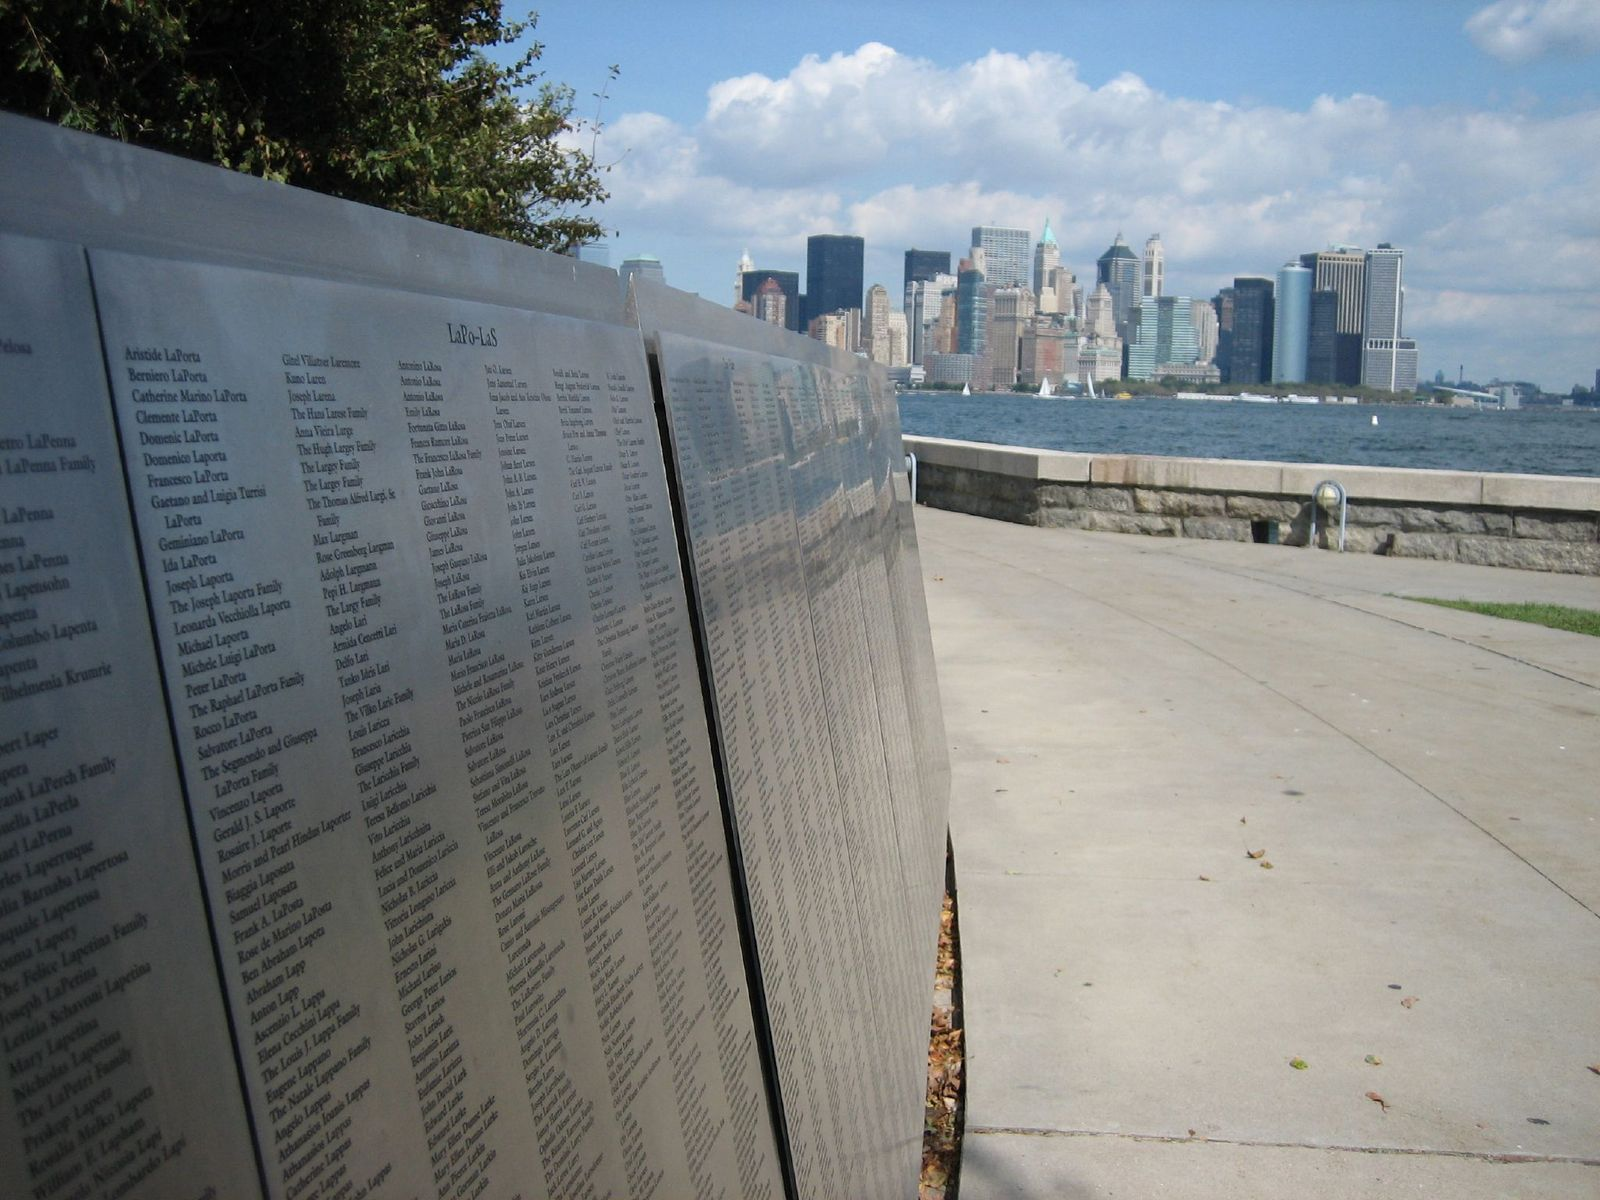
\includegraphics[width=.95\linewidth]{ellis0.jpg}
\end{subfigure}%
\begin{subfigure}{.5\textwidth}
  \centering
  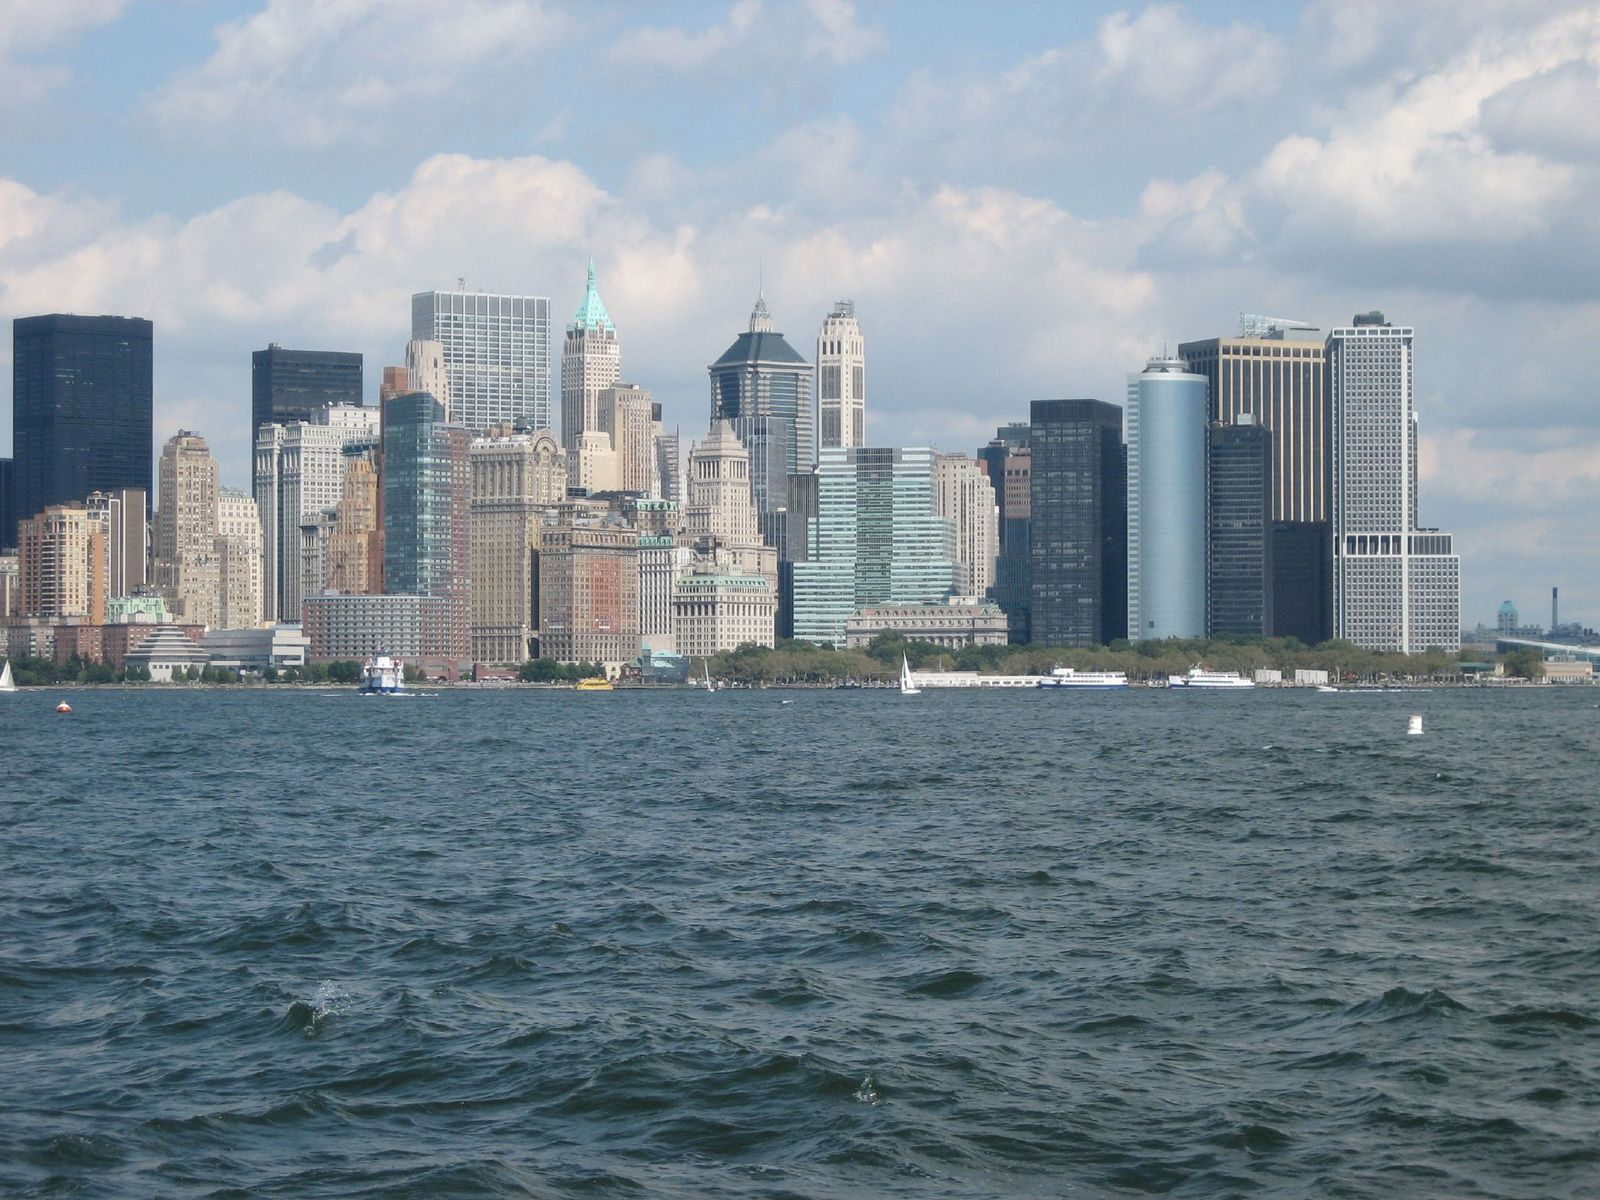
\includegraphics[width=.95\linewidth]{ellis1.jpg}
\end{subfigure}
\captionsetup{labelformat=empty}
\caption{Малюнак \arabic{figure}: набор дадзеных ellis}
\label{fig:ellis}
\end{figure}

\begin{table}[h]
  \centering
  \begin{footnotesize}
  \begin{tabular}{ | p{16mm} | p{17mm} | p{19mm} | p{22mm} | p{20mm} | p{22mm} | p{22mm} | }
    \hline
    Тып дэтэктара & Сярэдняя колькасць кропак & Час дэтэкцыі & Час на адну ключавую кропку & Тып дэскрыптара & Час на падлік дэскрыптараў & Час на падлік аднаго дэскрыптара \\ \hline
    SIFT & 2725 & 0.4967 & 0.0000911 & SIFT & 0.6985 & 0.0001281 \\ \hline
    SURF & 4950 & 0.4373 & 0.0000442 & SURF & 1.3399 & 0.0001353 \\ \hline
    BRISK & 3619 & 0.0883 & 0.0000122 & BRISK & 0.0716 & 0.0000099 \\ \hline
    ORB & 2947 & 0.0217 & 0.0000037 & ORB & 0.0240 & 0.0000041 \\ \hline
    AKAZE & 917 & 0.3723 & 0.0002029 & AKAZE & 0.2570 & 0.0001401 \\ \hline
    CenSurE & 261 & 0.0311 & 0.0000597 & BRIEF & 0.0023 & 0.0000044 \\ \hline
  \end{tabular}
  \end{footnotesize}
\captionsetup{labelformat=empty,justification=centering}
\caption{Табліца \arabic{table}: пошук асаблівых кропак і падлік адпаведных дэскрыптараў на наборы \textit{ellis}}
\label{table:ellis-kp}
\end{table}

\begin{table}[h]
  \centering
  \begin{footnotesize}
  \begin{tabular}{ | p{20mm} | p{22mm} | p{15mm} | p{22mm} | p{15mm} | p{22mm} | p{15mm} | }
    \hline
    Дэтэктар, дэскрыптар & BF адпаведнасцяў & BF час & BF-knn адпаведнасцяў & BF-knn час & FLANN адпаведнасцяў & FLANN час \\ \hline
    SIFT & 1265 & 0.8107 & 158 & 0.6754 & 142 & 0.0785 \\ \hline
    SURF & 1746 & 1.0627 & 149 & 1.0799 & 118 & 0.1052 \\ \hline
    BRISK & 1796 & 0.6418 & 93 & 0.6134 & 78 & 0.1154 \\ \hline
    ORB & 1469 & 0.1894 & 111 & 0.2477 & 92 & 0.0463 \\ \hline
    AKAZE & 494 & 0.0343 & 76 & 0.0368 & 58 & 0.0142 \\ \hline
    CenSurE+\newline BRIEF & 126 & 0.0017 & 9 & 0.0020 & 11 & 0.0015 \\ \hline
  \end{tabular}
  \end{footnotesize}
\captionsetup{labelformat=empty,justification=centering}
\caption{Табліца \arabic{table}: пошук адпаведнасцяў на наборы \textit{ellis}}
\label{table:ellis-matching}
\end{table}

\begin{figure}[H]
\centering
\begin{subfigure}{.5\textwidth}
  \centering
  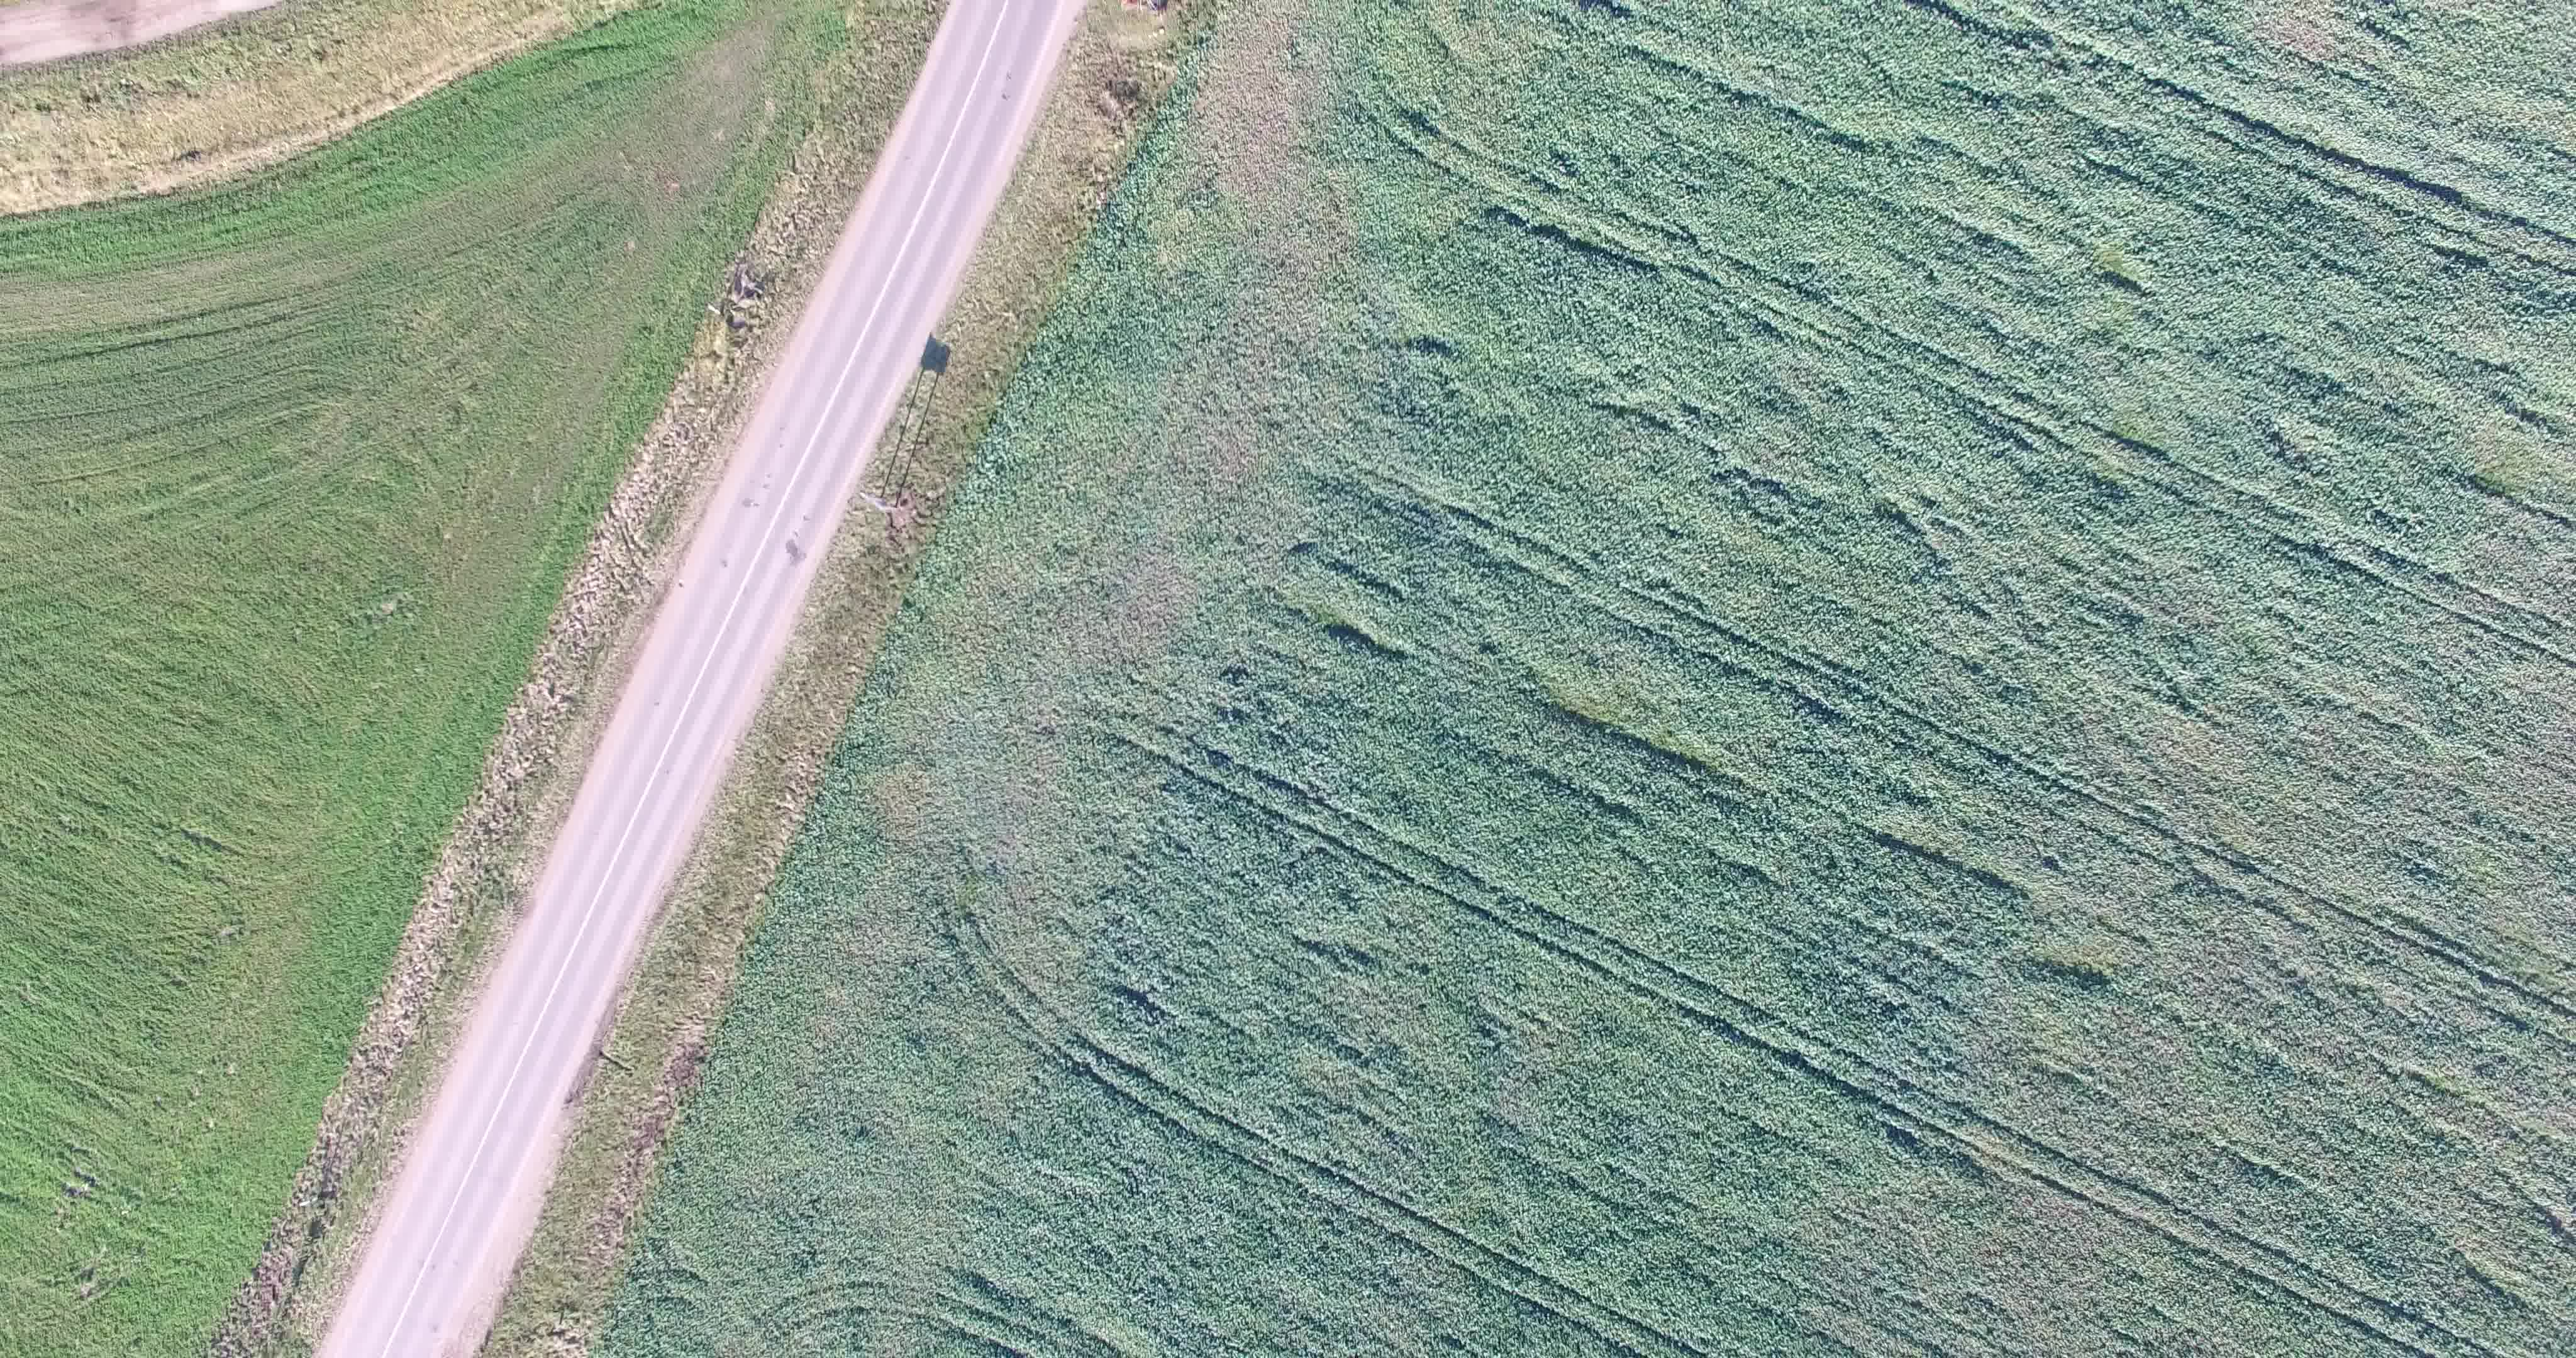
\includegraphics[width=.95\linewidth]{grass0.jpg}
\end{subfigure}%
\begin{subfigure}{.5\textwidth}
  \centering
  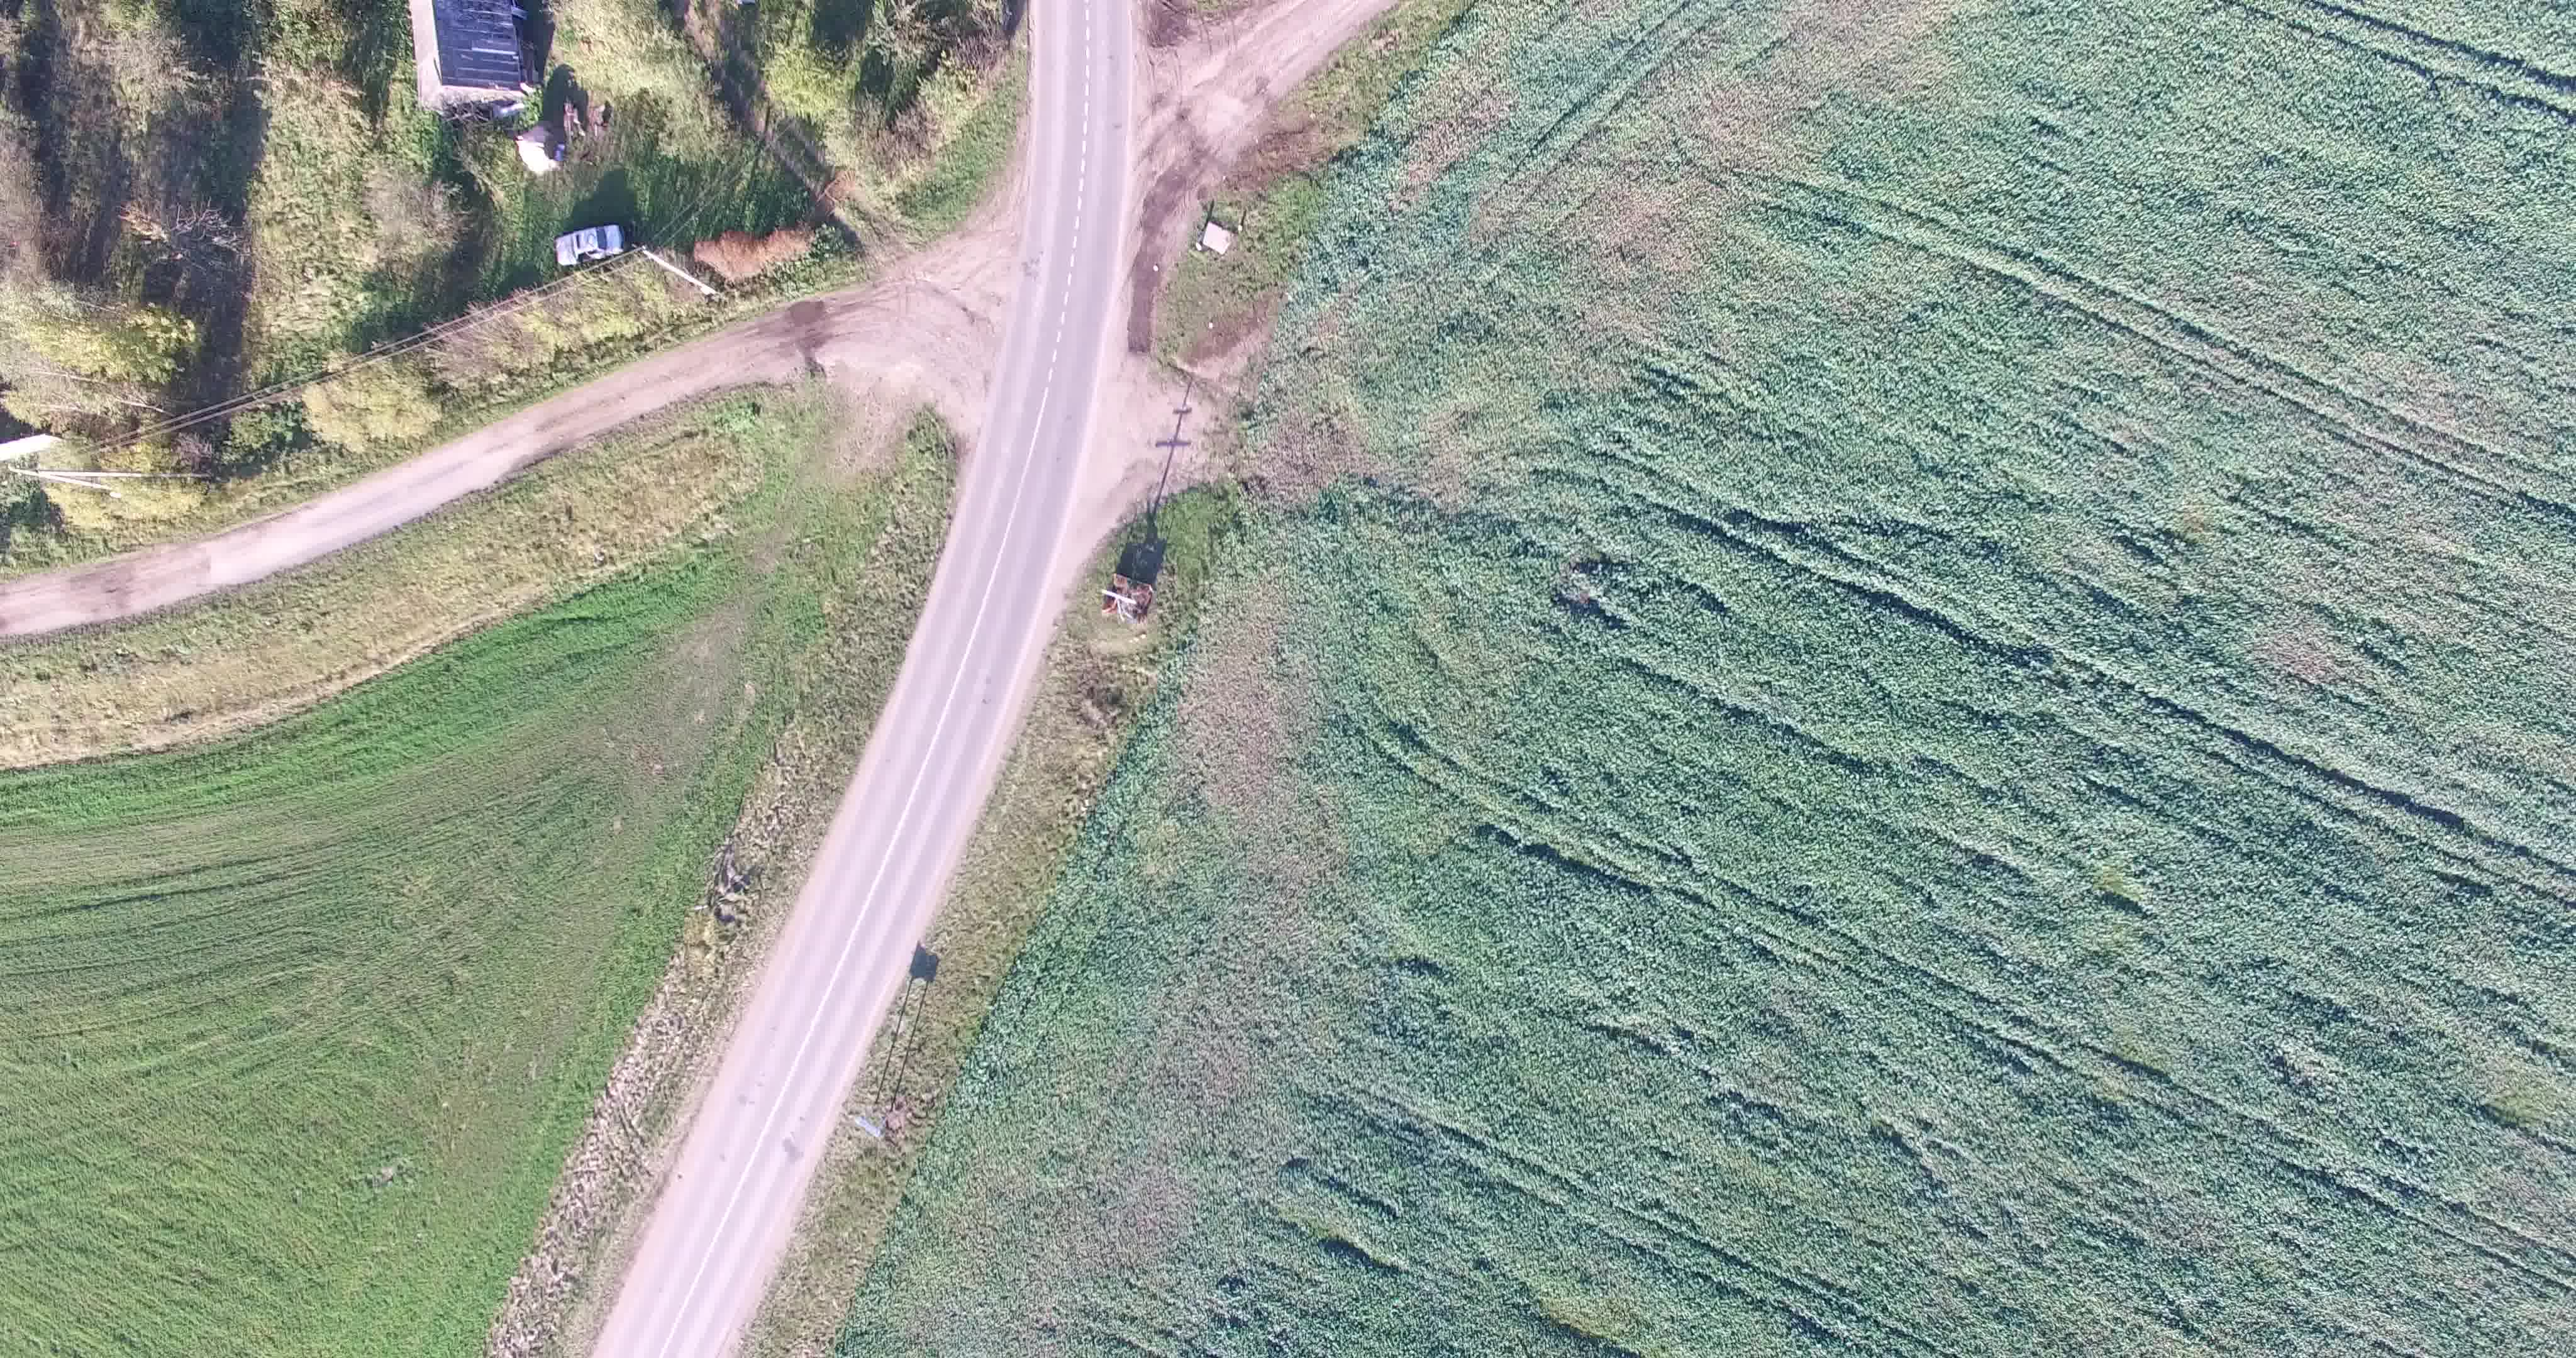
\includegraphics[width=.95\linewidth]{grass1.jpg}
\end{subfigure}
\captionsetup{labelformat=empty}
\caption{Малюнак \arabic{figure}: набор дадзеных grass}
\label{fig:grass}
\end{figure}

\begin{table}[h]
  \centering
  \begin{footnotesize}
  \begin{tabular}{ | p{16mm} | p{17mm} | p{19mm} | p{22mm} | p{20mm} | p{22mm} | p{22mm} | }
    \hline
    Тып дэтэктара & Сярэдняя колькасць кропак & Час дэтэкцыі & Час на адну ключавую кропку & Тып дэскрыптара & Час на падлік дэскрыптараў & Час на падлік аднаго дэскрыптара \\ \hline
    SIFT & 5357 & 0.6637 & 0.0000619 & SIFT & 0.9163 & 0.0000855 \\ \hline
    SURF & 15894 & 1.1313 & 0.0000356 & SURF & 3.5399 & 0.0001114 \\ \hline
    BRISK & 46305 & 1.3892 & 0.0000150 & BRISK & 0.8116 & 0.0000088 \\ \hline
    ORB & 3000 & 0.0921 & 0.0000154 & ORB & 0.0313 & 0.0000052 \\ \hline
    AKAZE & 3057 & 0.6880 & 0.0001125 & AKAZE & 0.7078 & 0.0001158 \\ \hline
    CenSurE & 829 & 0.1565 & 0.0000944 & BRIEF & 0.0199 & 0.0000120 \\ \hline
  \end{tabular}
  \end{footnotesize}
\captionsetup{labelformat=empty,justification=centering}
\caption{Табліца \arabic{table}: пошук асаблівых кропак і падлік адпаведных дэскрыптараў на наборы \textit{grass}}
\label{table:grass-kp}
\end{table}

\begin{table}[h]
  \centering
  \begin{footnotesize}
  \begin{tabular}{ | p{20mm} | p{22mm} | p{15mm} | p{22mm} | p{15mm} | p{22mm} | p{15mm} | }
    \hline
    Дэтэктар, дэскрыптар & BF адпаведнасцяў & BF час & BF-knn адпаведнасцяў & BF-knn час & FLANN адпаведнасцяў & FLANN час \\ \hline
    SIFT & 3043 & 2.6474 & 520 & 2.5827 & 452 & 0.1635 \\ \hline
    SURF & 8704 & 11.6172 & 848 & 11.5856 & 712 & 0.4455 \\ \hline
    BRISK & 24512 & 93.8451 & 1852 & 94.3301 & 1460 & 9.8551 \\ \hline
    ORB & 1624 & 0.2333 & 238 & 0.4267 & 207 & 0.1301 \\ \hline
    AKAZE & 1735 & 0.4762 & 732 & 0.4167 & 668 & 0.4133 \\ \hline
    CenSurE+\newline BRIEF & 452 & 0.0177 & 181 & 0.0188 & 172 & 0.0108 \\ \hline
  \end{tabular}
  \end{footnotesize}
\captionsetup{labelformat=empty,justification=centering}
\caption{Табліца \arabic{table}: пошук адпаведнасцяў на наборы \textit{grass}}
\label{table:grass-matching}
\end{table}

Кожны з набораў дадзеных апрацоўваўся шасцю рознымі алгарытмамі пошуку і падліку ключавых кропак.
Пры правядзенні эксперыменту была спроба прымянення і іншых алгарытмаў, якія не прысутнічаюць цяпер у табліцах,
аднак яны не паказалі вынікаў параўнальных з вышэй прыведзенымі. Напрыклад, натуральнай падавалася пара дэтэктар FAST і
дэскрыптар ORB, якая, аднак, паказала кепскія вынікі як па часе, так і па якасці знойдзеных адпаведнасцяў.

Прывядзем апісанне ўжытых метадаў пошука адпаведнасцяў згодна з іх скарачэннямі ў табліцах:
\begin{itemize}
  \item \textit{BF} - звычайны BruteForce алгарытм, рэалізацыя з OpenCV, запускаўся з параметрам \textit{CrossCheck = True}:
  гэты параметр кажа алгарытму вяртаць пару спалучаных дэскрыптараў толькі тады, калі кожны з дэскрыптараў на чарговым кроку
  выступае найлепшым для свайго адпаведніка на іншай выяве (то бок дэскрыптары павінны спалучацца ``у абодва бакі''). Гэта з'яўляецца
  своеасаблівай альтэрнатывай ``тэсту суадносінаў'' (англ. \textit{ratio test}),
  апісанаму ў \cite{sift-paper} - гэты тэст мы будзем запускаць разам з наступным метадам.
  \item \textit{BF-knn} - BruteForce алгарытм, які структуруе знойдзеныя адпаведнасці крыху іншым чынам, чым вышэйзгаданы BF:
  для кожнага дэскрыптара ён знаходзіць не больш за $k=2$ адпаведных дэскрытараў. Далей мы запускаем ``тэст суадносінаў'',
  які апісаны ў \cite{sift-paper} (старонка 20). Сцвярджаецца, што калі адлегласці двух найлепшых знойдзеных адпаведнікаў для
  вызначанага дэскрыптара адпавядаюць няроўнасці $distance_1 < ratio \times distance_2$, дзе $ratio$ - канстанта, якая звычайна
  абіраецца з прамежка $[0.7, 0.8]$, то першы адпаведнік для знойдзенага дэскрыптара з'яўляецца ``дастаткова добрым'' - такія дэскрыптары
  заносяцца ў табліцу як ``знойдзеныя''. Трэба заўважыць, што гэты ``тэст суадносінаў'' на практыцы праходзіць дастаткова мала
  параў дэскрыптараў.
  \item \textit{FLANN} - сямейства алгарытмаў набліжанага пошуку бліжэйшых суседзяў. У нашым выпадку, для SIFT i SURF гэты алгарытм
  заснаваны на KD-дрэвах, для астатніх дэскрыптараў гэта LSH (Locality-sensitive hashing).
\end{itemize}

Заўвагі:
\begin{itemize}
  \item алгарытм ORB прымае ў якасці аднаго з параметраў абмежаванне зверху на колькасць знойдзеных ключавых кропак;
  у табліцах \ref{table:church-kp} - \ref{table:grass-matching}, калі колькасць ключавых кропак, знойдзеных ORB, роўная 3000,
  гэта не азначае, што гэта максімальна магчымы лік; для астатніх алгарытмаў прыведзеныя максімальныя значэнні.
\end{itemize}

На малюнках \ref{fig:matches1} - \ref{fig:matches2} прыведзеныя два прыклады знойдзеных адпаведнасцяў. Колькасць нанесеных
у выглядзе лініяў адпаведнасцяў абмежаваная лікам 20 для паляпшэння нагляднасці.

\begin{figure}[H]
  \centering
  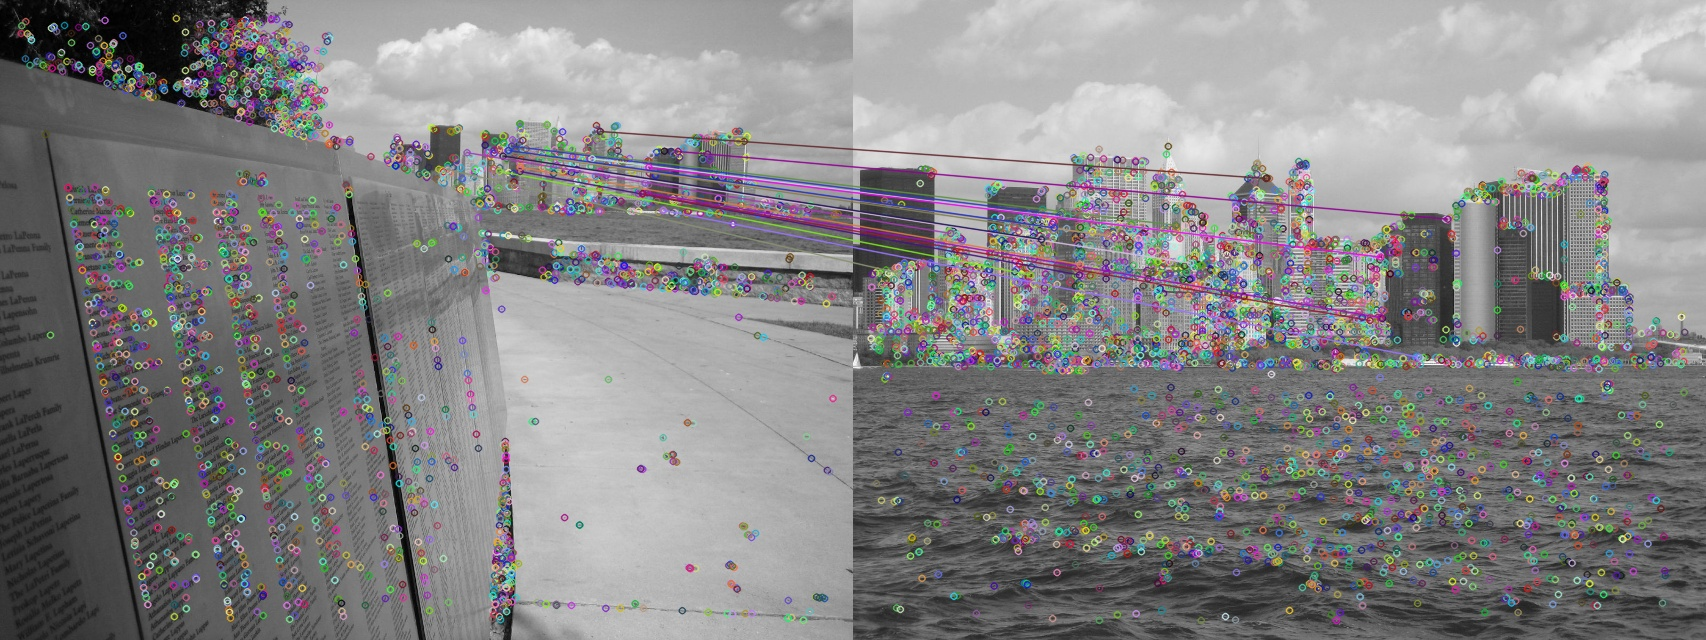
\includegraphics[width=.9\textwidth]{matches/ellis_BRISK_bf_crossCheck_matches.jpg}
  \captionsetup{labelformat=empty}
  \caption{Малюнак \arabic{figure}: знойдзеныя адпаведнасці (ellis, BRISK, BF)}
  \label{fig:matches1}
\end{figure}

\begin{figure}[H]
  \centering
  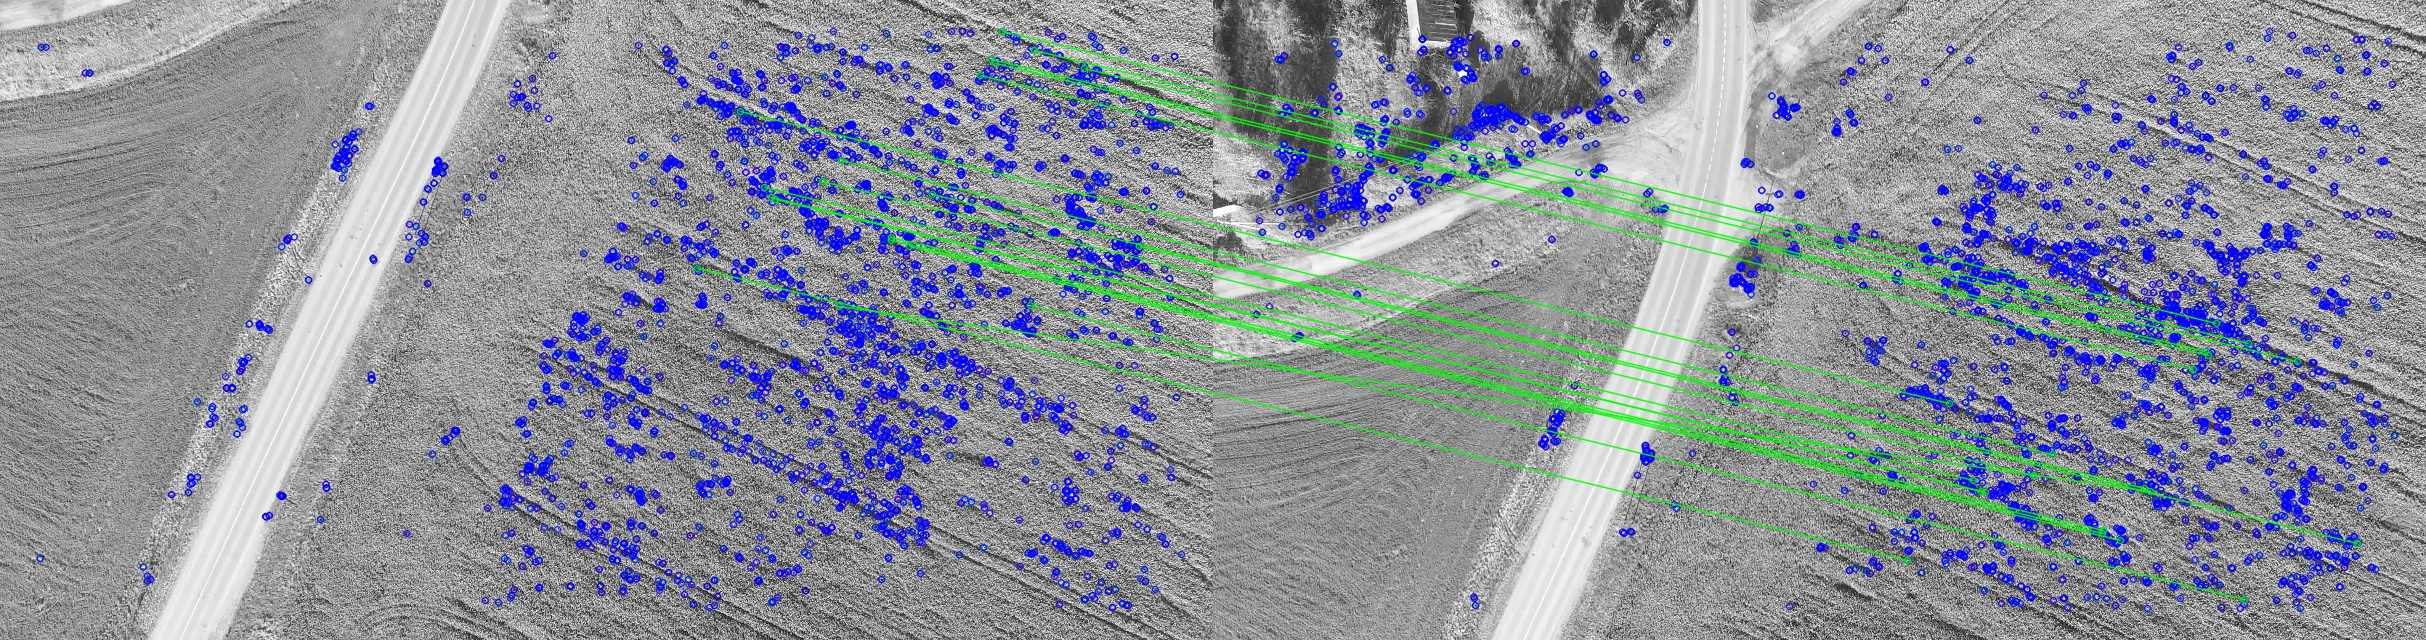
\includegraphics[width=.9\textwidth]{matches/grass_ORB_flann_knn_matches.jpg}
  \captionsetup{labelformat=empty}
  \caption{Малюнак \arabic{figure}: знойдзеныя адпаведнасці (grass, ORB, FLANN)}
  \label{fig:matches2}
\end{figure}

Высновы:
\begin{itemize}
  \item Алгарытмы дастаткова яскрава падзяліліся на ``хуткія'' і ``марудныя''. ORB заўсёды хутчэй за ўсіх знаходзіць
  ключавыя кропкі і падлічвае для іх дэскрыптары (часам гэтаму спрыяе штучнае абмежаванне ў 3000 на колькасць
  ключавых кропак). Пошук адпаведнасцяў таксама заўсёды адбываецца хутка (у параўнанні з іншым алгарытмамі),
  хаця і моцна вар'юецца: ад 0.02с да 0.4с.
  \item Пара алгарытмаў CenSurE+BRIEF знаходзіць малую колькасць ключавых кропак (часам на парадак менш, чым іншыя
  алгарытмы на тых жа наборах дадзеных), прычым па часе могуць прайграць таму ж ORB. Негледзячы на гэта, маленькая
  колькасць дазваляе вельмі хутка знаходзіць адпаведнасці.
  \item Алгарытм BRISK кепска прымяняецца да аднастайных дадзеных: на наборы \textit{grass} колькасць знойдзеных ключавых кропак
  рэзка ўзрастае (у ~3 разы больш за наступны па колькасці знойдзеных кропак алгарытм). На іншых наборах дадзеных BRISK
  паводзіць сябе зусім іншым чынам. У выніку алгарытм выкарыстаў рэкордны для нашага даследвання час на на пошук асаблівасцяў
  (~94c на BF i BF-knn). Трэба сказаць, што падобныя паводзіны за BRISK-ам былі заўважаныя і на іншых выявах
  са слабай тэкстураванасцю.
  \item У агульным выпадку можна казаць пра маруднасць алгарытма SURF на этапе падліку дэскрыптараў: на ўсіх чатырох
  наборах ён падлічваў значэнні дэскрыптараў з самым вялікім абсалютным значэннем па часе, і быў адным з самых
  марудных у пераліку на час на адзін дэскрыптар.
\end{itemize}

Агульнае падсумаванне можна сфармуляваць наступным чынам: існуюць алгарытмы для хуткай апрацоўкі і для больш грунтоўнай,
алгарытмы, якія паказваюць падобныя вынікі на любых дадзеных і алгарытмы, слаба прымяняльныя на канкрэтных дадзеных.
SIFT i SURF можна ўмоўна аднесці да надзейных, але марудных: яны часта выкарыстоўваюцца на прыладах з добрымі характарыстыкамі,
але радзей знаходзяць сваё прымяненне да мабільных прыладах. Нагадаем, што абодва гэтыя алгарытмы апісваюць ключавыя кропкі
пры дапамозе рэчаісных вектароў, што, вядома, марудней за бінарныя радкі.
Ва ўмовах абмежаваных рэсурсаў часта знаходзяць сваё прымяненне
алгарытмы ORB i AKAZE: у нашых лічбах яны з'яўляюцца найхутчэйшымі і найменш залежнымі ад рэсурсаў.
BRISK паводзіць сябе на ўзроўні іншых алгарытмаў (па колькасных і часавых характарыстыках), але на такіх наборах, як
\textit{church} альбо \textit{grass} паказвае рэзкае адставанне па часе на этапе пошуку адпаведнасцяў праз вялікую колькасць
папярэдне вылучаных асаблівых кропак.

Цікаўнасць для даследвання прадстаўляе таксама хуткасць роста ад дыстанцыі ў адсартаваных масівах знойдзеных адпаведнасцяў.
Дыстанцыя, па сутнасці, з'яўляецца непасрэднай характарыстыкай якасці знойдзенай адпаведнасці, а таксама проста ўплывае на тое,
ці пройдзе пара ``тэст суадносінаў'', які апісываўся вышэй.

На графіках \ref{fig:best20matches} - \ref{fig:best250matches} прадстаўленыя адлегласці лепшых адпаведна 20 і 250 параў дэскрыптараў.
Пары былі суаднесеныя BF алгарытмам. Дадзеныя на графіках палічаныя адносна апошняй (адпаведна, 20ай альбо 250ай) адлегласці.
Інтэрпрэтуюцца дадзеныя наступным чынам: рэзкі рост графіка абазначае рэзкі рост кожнай наступнай адлегласці, адпаведна - адлегласць
паміж кожнай наступнай парай дэскрыптараў значна больш. Разам з тым, больш спадзісты характар графіка сведчыць пра нізкі рост
у значэннях адлегласцяў. На графіках часцей за ўсё асобна выбіваецца AKAZE - у табліцах \ref{table:church-kp} - \ref{table:grass-matching}
гэта адлюстроўваецца ў тым, што на некаторых наборах дадзеных суадносіны ``колькасць адпаведнасцяў знойдзеных BF-knn да пачатковай
колькасці дэскрыптараў'' для AKAZE найвялікшая.

\begin{figure}[h]
\centering
\begin{subfigure}{.5\textwidth}
  \centering
  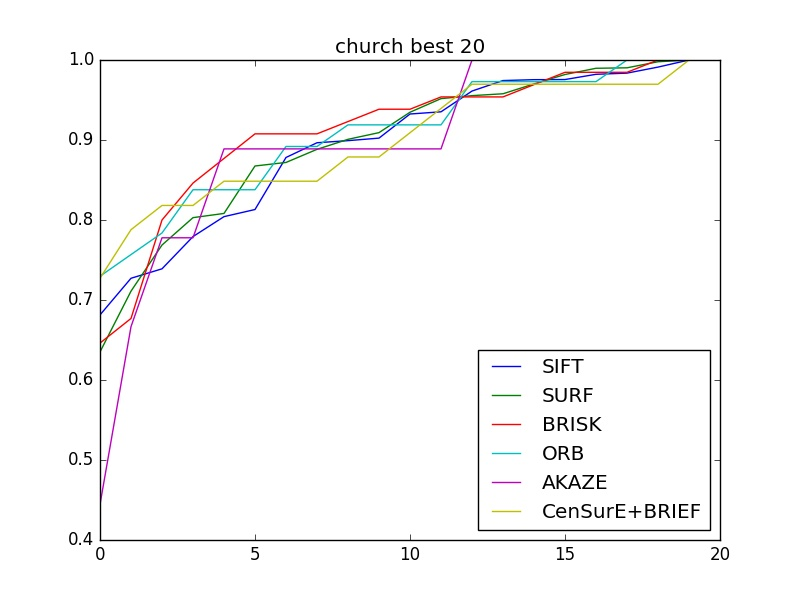
\includegraphics[width=\linewidth]{graphs/church_top20.jpg}
  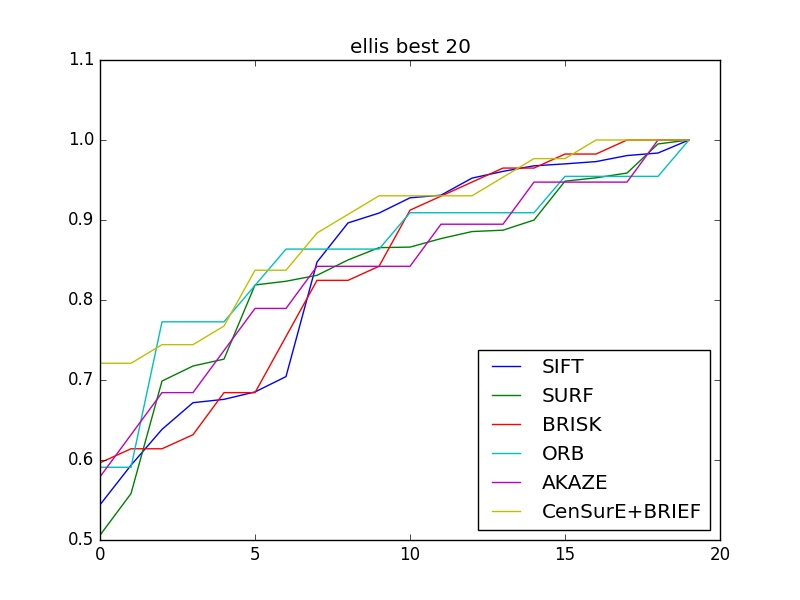
\includegraphics[width=\linewidth]{graphs/ellis_top20.jpg}
\end{subfigure}%
\begin{subfigure}{.5\textwidth}
  \centering
  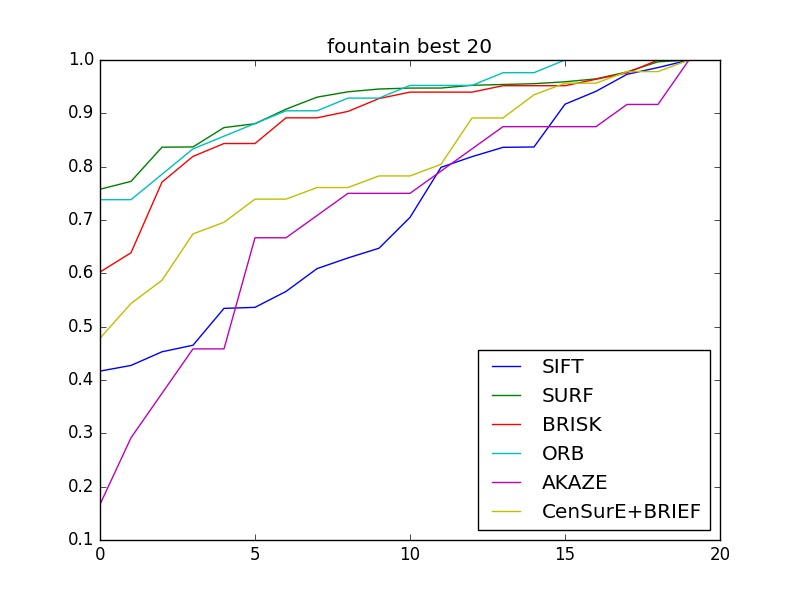
\includegraphics[width=\linewidth]{graphs/fountain_top20.jpg}
  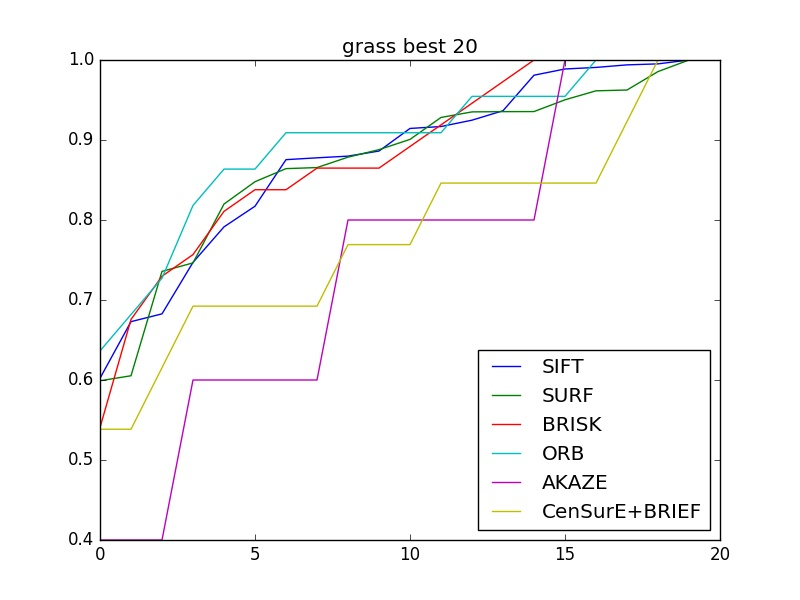
\includegraphics[width=\linewidth]{graphs/grass_top20.jpg}
\end{subfigure}%
\captionsetup{labelformat=empty,justification=centering}
\caption{Малюнак \arabic{figure}: рост адлегласці ў 20 лепшых парах}
\label{fig:best20matches}
\end{figure}

\begin{figure}[h]
\centering
\begin{subfigure}{.5\textwidth}
  \centering
  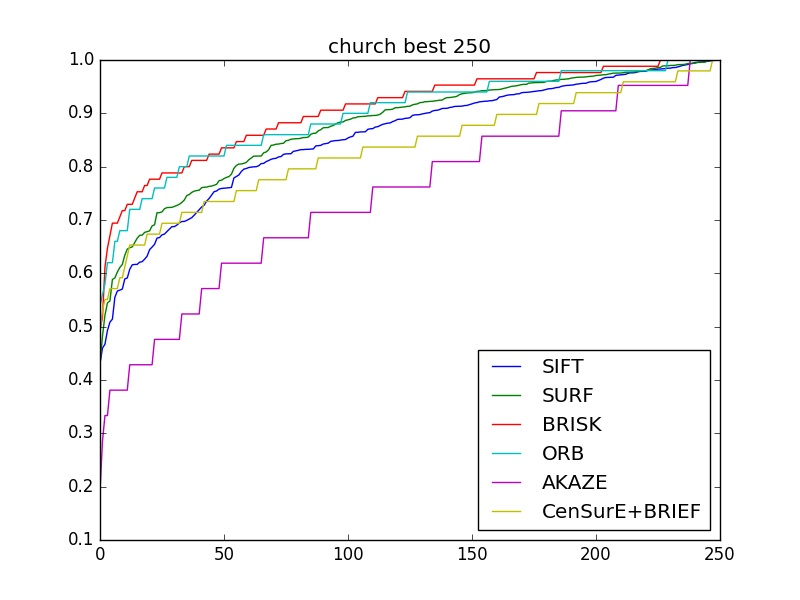
\includegraphics[width=\linewidth]{graphs/church_top250.jpg}
  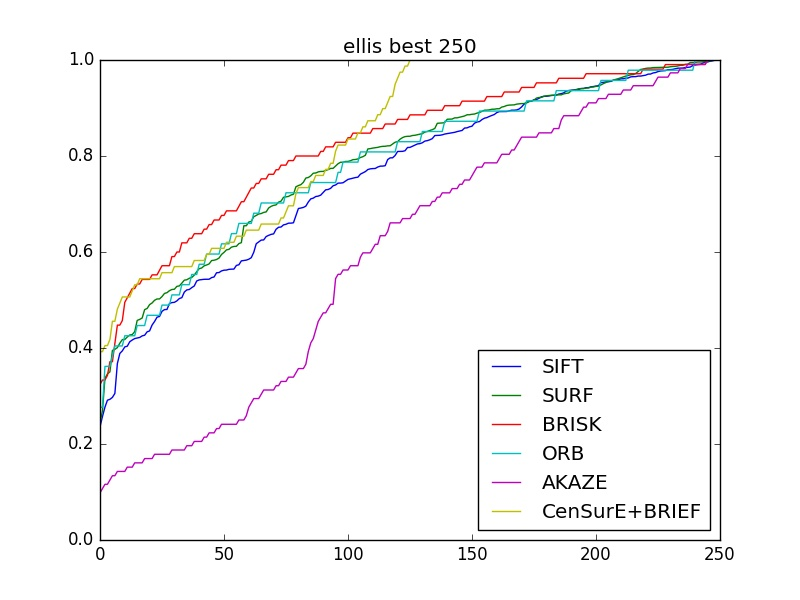
\includegraphics[width=\linewidth]{graphs/ellis_top250.jpg}
\end{subfigure}%
\begin{subfigure}{.5\textwidth}
  \centering
  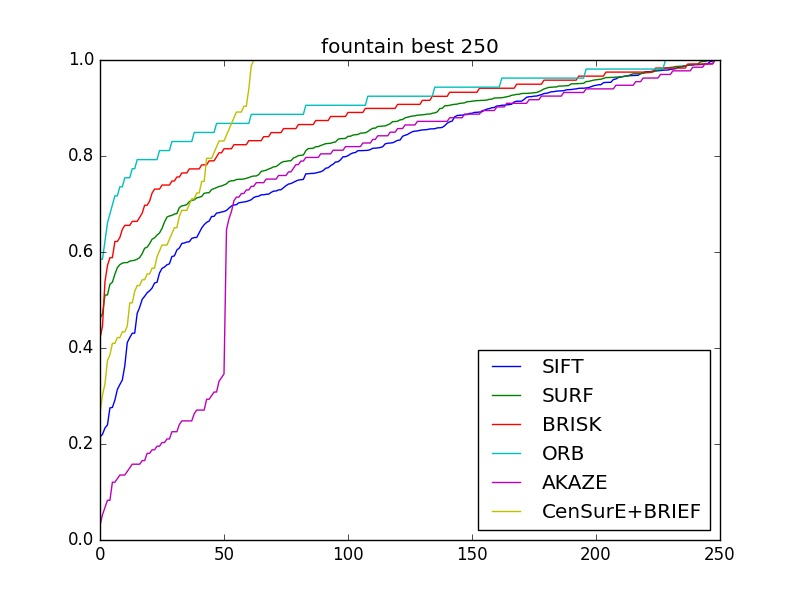
\includegraphics[width=\linewidth]{graphs/fountain_top250.jpg}
  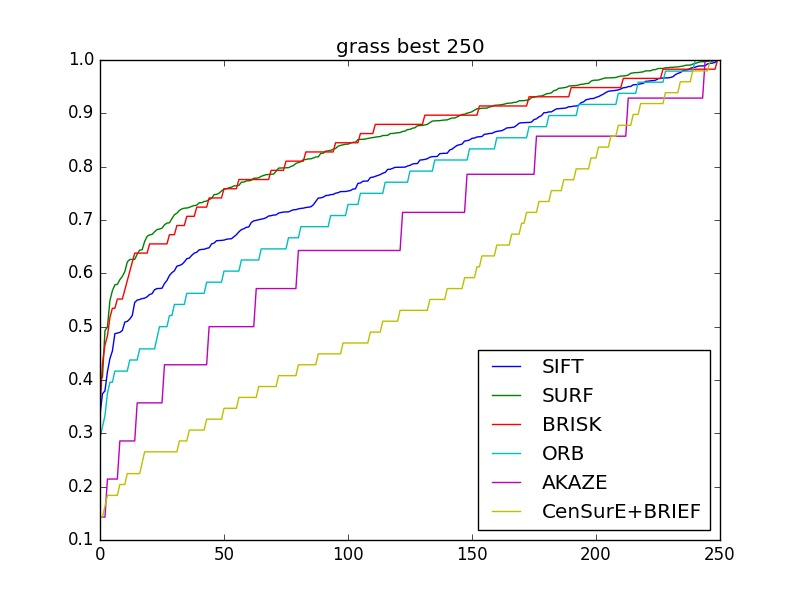
\includegraphics[width=\linewidth]{graphs/grass_top250.jpg}
\end{subfigure}%
\captionsetup{labelformat=empty,justification=centering}
\caption{Малюнак \arabic{figure}: рост адлегласці ў 250 лепшых парах}
\label{fig:best250matches}
\end{figure}

%
%
% APPA
%
%

\addcontentsline{toc}{subsection}{Распрацоўка праграмнага забеспячэння для рэканструкцыі паверхні}
\subsection*{2.2 Распрацоўка праграмнага забеспячэння для рэканструкцыі паверхні}

Асноўнай практычнай часткай маёй курсавой працы была рэалізацыя канечнай праграмы для рэканструкцыі паверхні па дадзеных
з БПЛА. Праграма напісаная на мове C++ з выкарыстаннем фрэймворка Qt на базе бібліятэкі камп'ютарнага зроку
з адкрытым зыходным кодам TheiaSfm \cite{theia-sfm}. Праграма
знаходзіцца ў актыўнай распрацоўцы, на дадзены момант рэалізаваныя ўсе асноўныя магчымасці, такія як адкрыццё/стварэнне новых праэктаў,
пабудова разрэджанага воблака кропак па наборы выяваў, трохмерная візуалізацыя мадэлі, падсветка выбранай камеры, паўторнае выкарыстанне
дадзеных (напрыклад, здзейсніўшы адзін раз пошук ключавых кропак, наступны раз гэты этап можа быць прапушчаны, што моцна эканоміць час
і рэсурсы), генерацыя справаздачаў пасля рэканструкцыі. Праграма працуе як у кансольным рэжыме, так і ў рэжыме з графічным
інтэрфейсам.

Праграма ствараецца з практычнымі метадамі: яна будзе карысная як для пабудовы мадэлі канечным карыстачом (выкарыстоўваючы
графічны інтэрфейс), так і, напрыклад, для правядзення эксперыментаў з алгарытмамі (у гэтым выпадку карыснай будзе магчымасць
выклікаць увесь функцыянал праграмы з кансольнага радка).

Праграма кросплатформенная, праца ўсяго функцыяналу была пратэставаная на аперацыйных сістэмах macOS i Ubuntu.

Здымкі экрана з запушчаным прыкладаннем прадстаўленыя на малюнках \ref{fig:screenshot1} - \ref{fig:screenshot3}.

\begin{figure}[H]
  \centering
  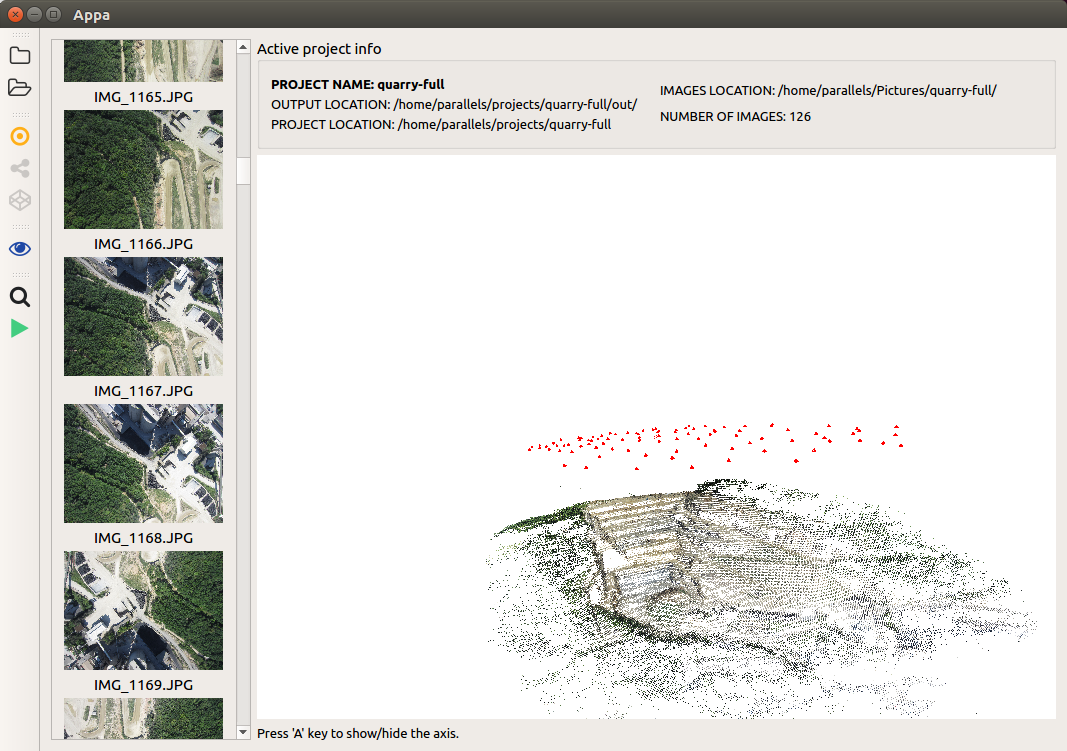
\includegraphics[width=.9\textwidth]{appa0.png}
  \captionsetup{labelformat=empty}
  \caption{Малюнак \arabic{figure}: здымак экрана}
  \label{fig:screenshot1}
\end{figure}

\begin{figure}[H]
  \centering
  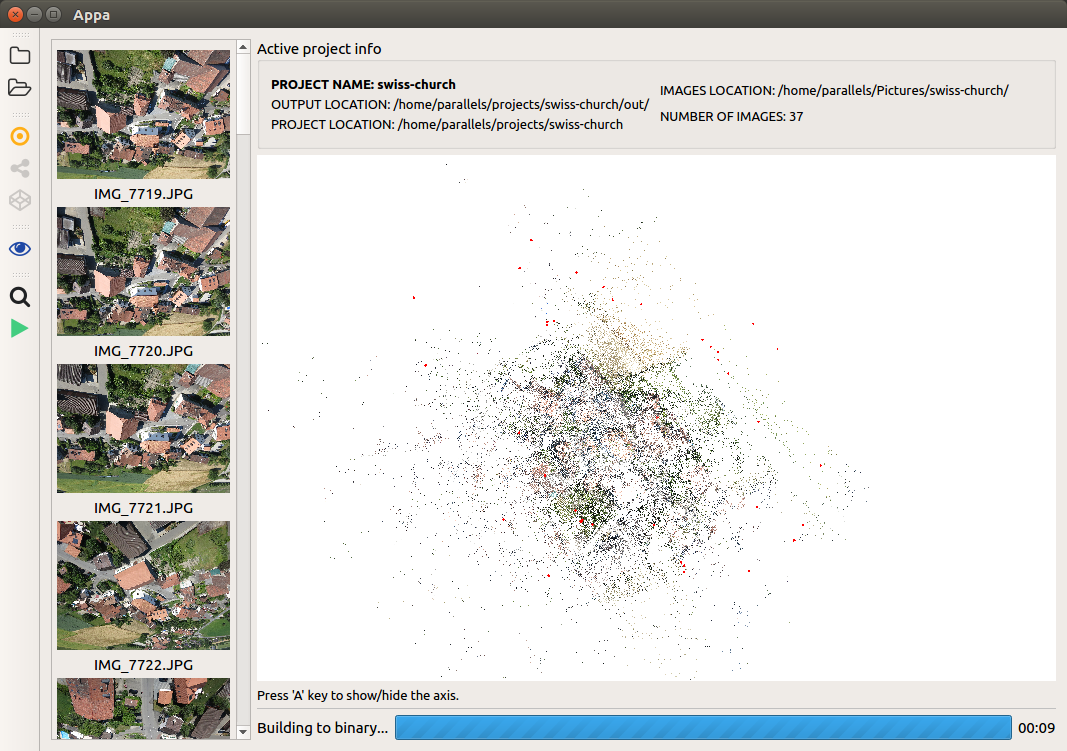
\includegraphics[width=.9\textwidth]{appa1.png}
  \captionsetup{labelformat=empty}
  \caption{Малюнак \arabic{figure}: здымак экрана}
  \label{fig:screenshot2}
\end{figure}

\begin{figure}[H]
  \centering
  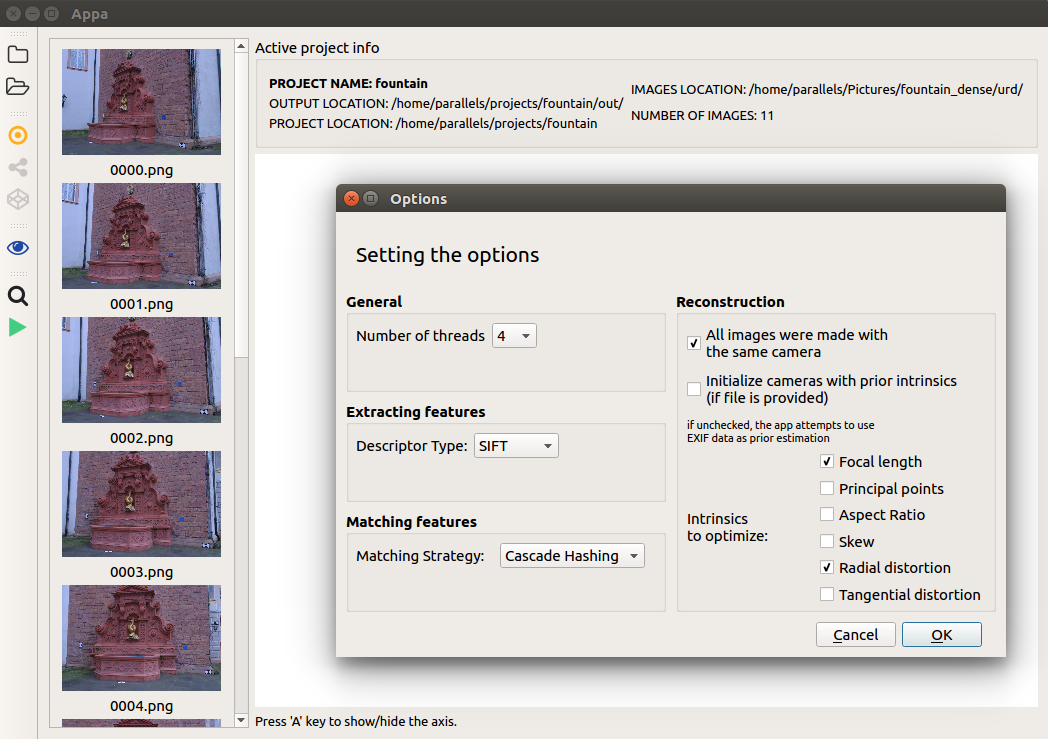
\includegraphics[width=.9\textwidth]{appa2.png}
  \captionsetup{labelformat=empty}
  \caption{Малюнак \arabic{figure}: здымак экрана}
  \label{fig:screenshot3}
\end{figure}

Увесь зыходны код адкрыты і размешчаны на GitHub.

\newpage
